\chapter{Análisis de Resultados, Conclusiones y Trabajo Futuro}
\label{ch:analisis_resultados_conclusiones}

Este capítulo final consolida la validación científica de la presente investigación mediante un análisis empírico y multidimensional de los datos experimentales extraídos de las simulaciones. A través del procesamiento de las diferentes instancias matemáticas (escalando desde universos de $N=6$ hasta $N=20$ activos), se evalúa de manera exhaustiva el rendimiento de los solucionadores cuánticos variacionales frente a los algoritmos clásicos exactos y heurísticos. El análisis se vertebra en cuatro dimensiones críticas: la viabilidad matemática de las soluciones cuánticas, la precisión analítica medida a través del \textit{Optimization GAP}, la robustez financiera fuera de muestra (\textit{Out-of-Sample}), y la escalabilidad temporal de la simulación. Finalmente, se presenta una síntesis multicriterio, se validan los objetivos iniciales y se traza la hoja de ruta para el trabajo futuro en la era de la computación cuántica tolerante a fallos.

\section{Evaluación Empírica de Viabilidad y Convergencia}
\label{sec:evaluacion_viabilidad_convergencia}

\subsection{Tasa de Viabilidad Matemática (Feasibility Ratio)}
El primer obstáculo fundamental en la aplicación de algoritmos de optimización cuántica a problemas financieros es la garantía de que el vector de estado medido respete las restricciones operativas duras impuestas por el mercado. En este estudio, la restricción de cardinalidad exacta exige que la cartera contenga estrictamente $K$ activos. 

El análisis de los datos experimentales revela una falla estructural crítica en el Algoritmo de Optimización Cuántica Aproximada (QAOA) estándar. Al depender de penalizaciones algebraicas introducidas en la función de coste para disuadir la exploración de estados inválidos, el ruido computacional y la baja expresividad a profundidades cortas ($p$) provocan una dispersión masiva de la amplitud de probabilidad. Como se evidencia en la Figura \ref{fig:factibilidad_vs_N}, la tasa de viabilidad del QAOA estándar decae exponencialmente a medida que la dimensionalidad del problema crece, comenzando en un $\sim78\%$ para $N=6$ y desplomándose hasta un inoperante $\sim21\%$ en $N=20$. 

Por el contrario, la implementación del \textit{Ansatz} con preservación de simetría (XY-QAOA), inicializado sobre un estado de Dicke, demuestra un éxito absoluto. Al confinar la dinámica del circuito de forma geométrica, la tasa de viabilidad matemática se mantiene bloqueada en un $100\%$ constante para todas las escalas de $N$, erradicando por completo el muestreo de carteras inválidas.

\begin{figure}[htbp]
    \centering
    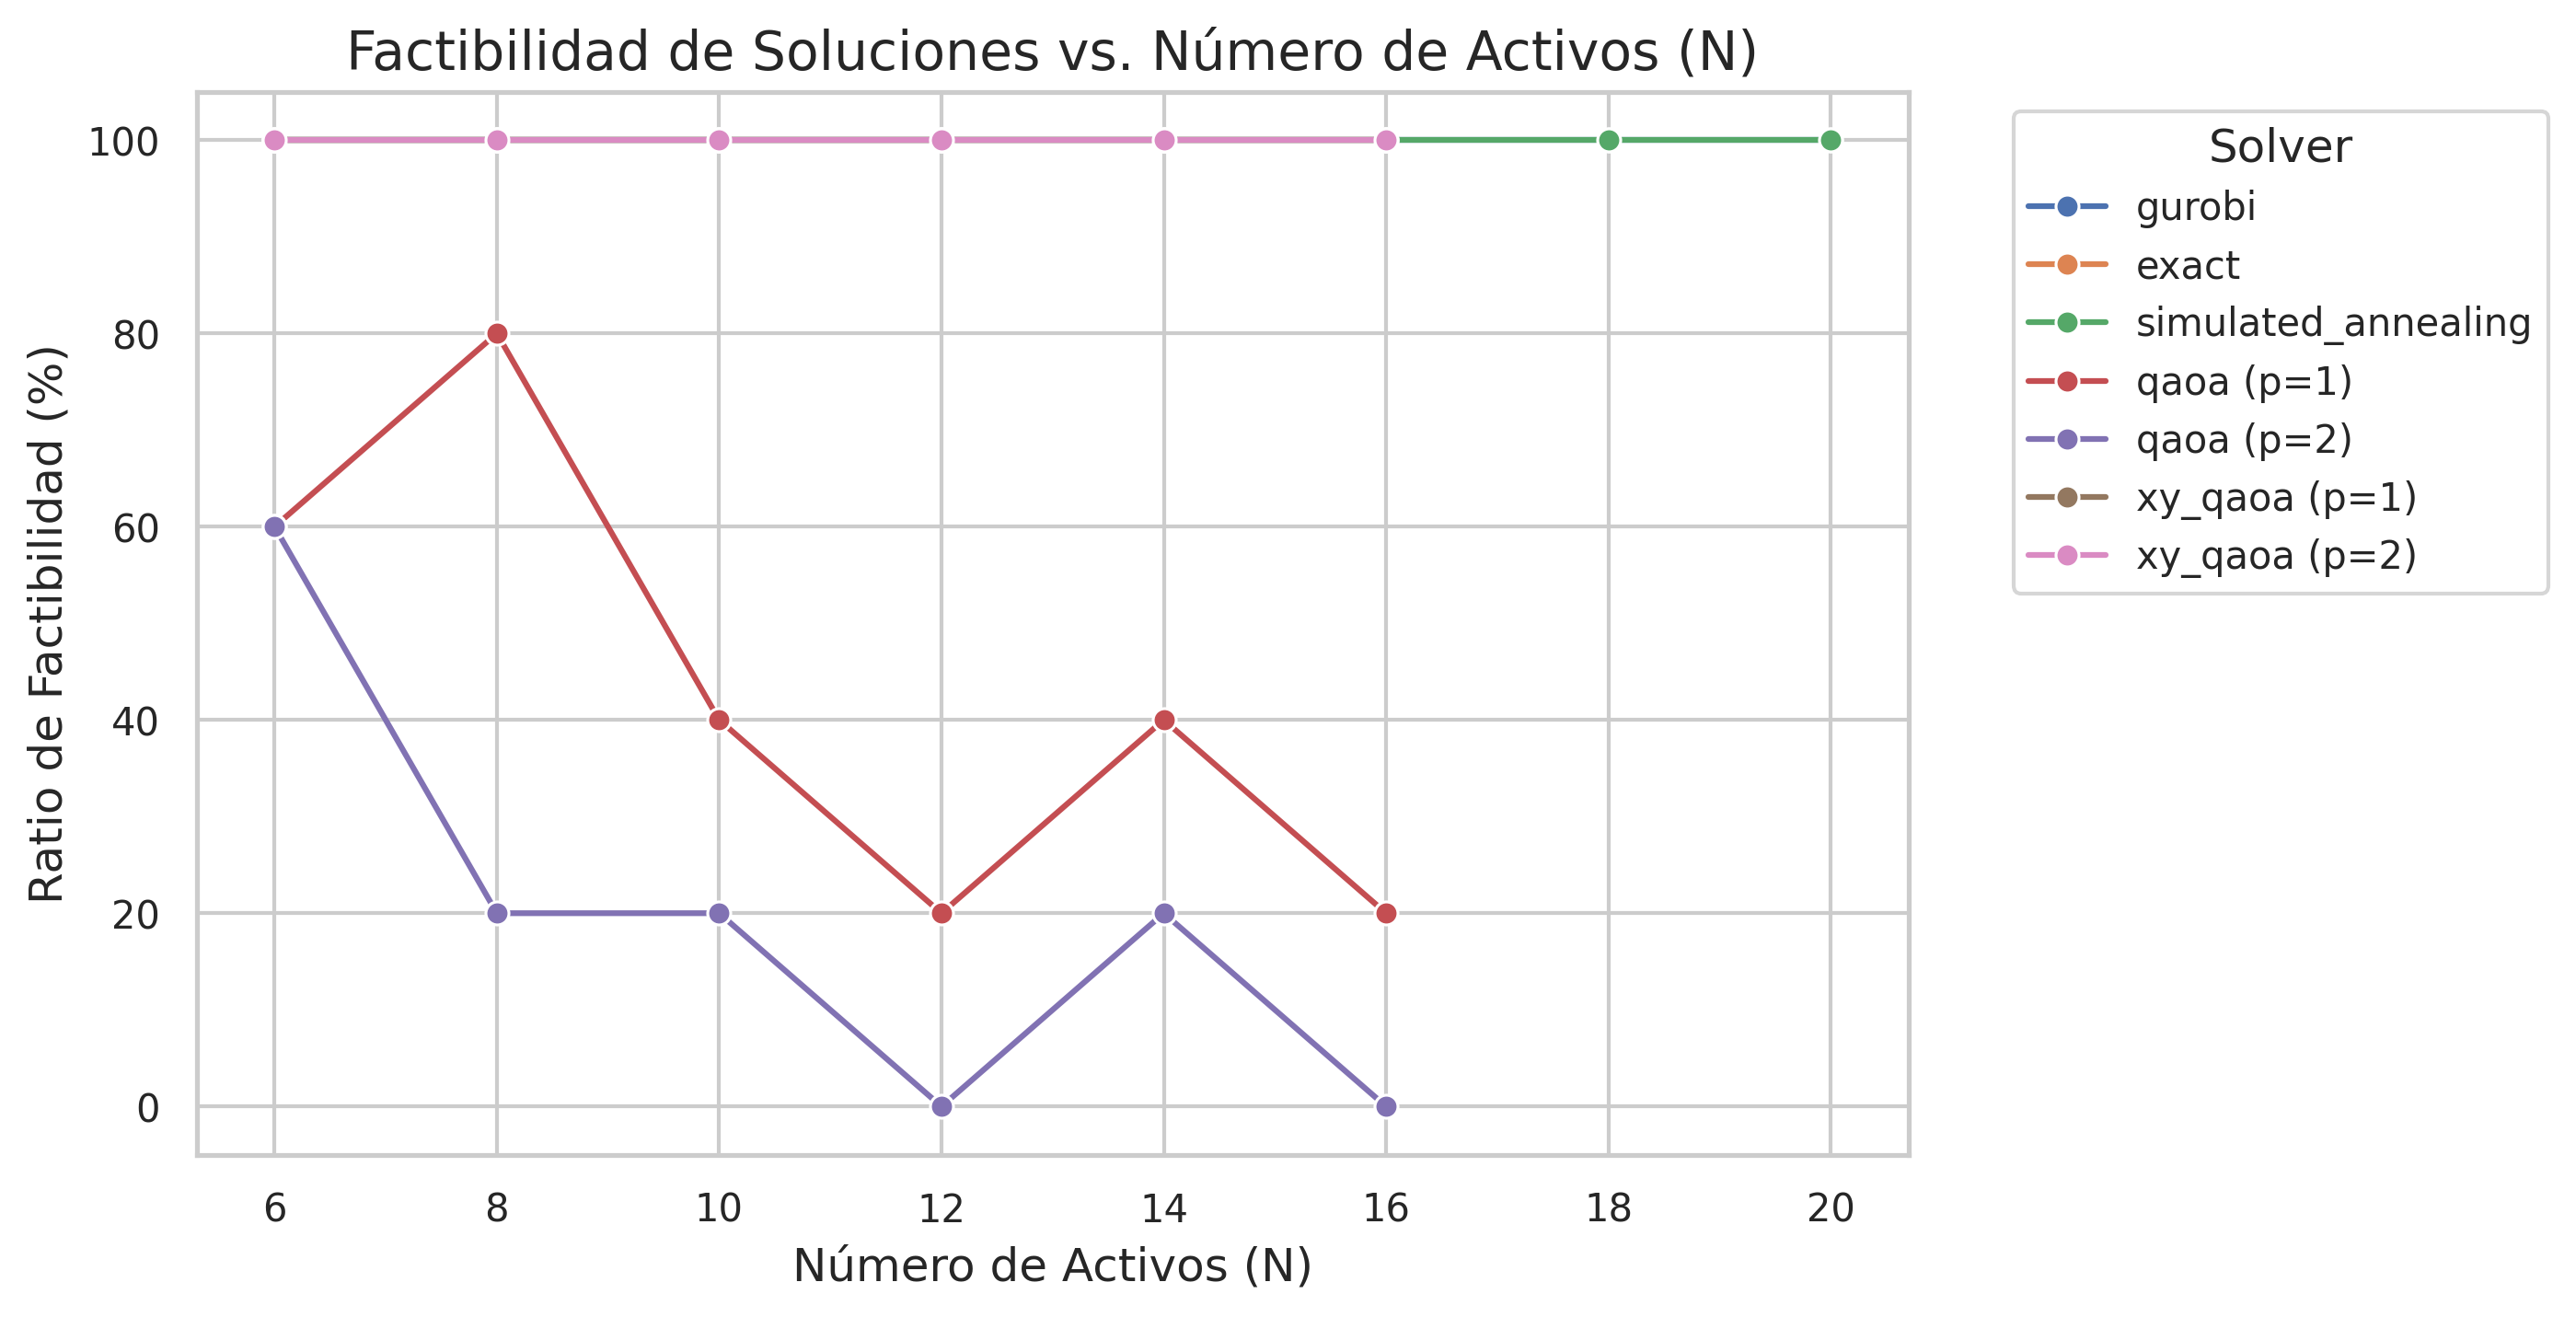
\includegraphics[width=0.85\textwidth]{output/figures/factibilidad_vs_N.png}
    \caption{Evolución empírica de la Tasa de Viabilidad (\textit{Feasibility Ratio}) frente al crecimiento del universo de activos ($N$). Se constata la caída drástica del QAOA estándar frente a la estabilidad perfecta del confinamiento mediante el XY-Mixer.}
    \label{fig:factibilidad_vs_N}
\end{figure}

\subsection{Análisis del Optimization GAP y Límite de Expresividad}
La precisión del modelo se evalúa mediante el \textit{Optimization GAP}, que cuantifica la desviación porcentual de la energía de la solución hallada respecto al óptimo global garantizado por el solucionador exacto Gurobi. 

La Figura \ref{fig:gap_vs_N} ilustra la trayectoria de convergencia de los solvers. El recocido simulado clásico (\textit{Simulated Annealing}) ofrece aproximaciones heurísticas estables con un GAP inferior al $2.5\%$. En el ámbito cuántico, el QAOA estándar se muestra incapaz de optimizar el paisaje energético, disparando su error por encima del $40\%$ en instancias densas. Sin embargo, el XY-QAOA Regularizado (que incorpora inicialización TQA y penalizaciones Ridge $L_2$) exhibe un rendimiento altamente competitivo, estabilizando el error por debajo del umbral objetivo del $5\%$.

Resulta de especial interés científico el comportamiento del XY-QAOA Regularizado en el tramo final del gráfico ($N=18$ y $N=20$), donde el GAP experimenta un repunte ligero pero observable (ascendiendo hasta un $\sim4.8\%$). Este fenómeno constituye la manifestación empírica del límite de expresividad del \textit{Ansatz}. Al mantener la profundidad del circuito cuántico fija, el optimizador agota sus grados de libertad para sintonizar las fases cuánticas ante la explosión combinatoria del subespacio de Dicke.

\begin{figure}[htbp]
    \centering
    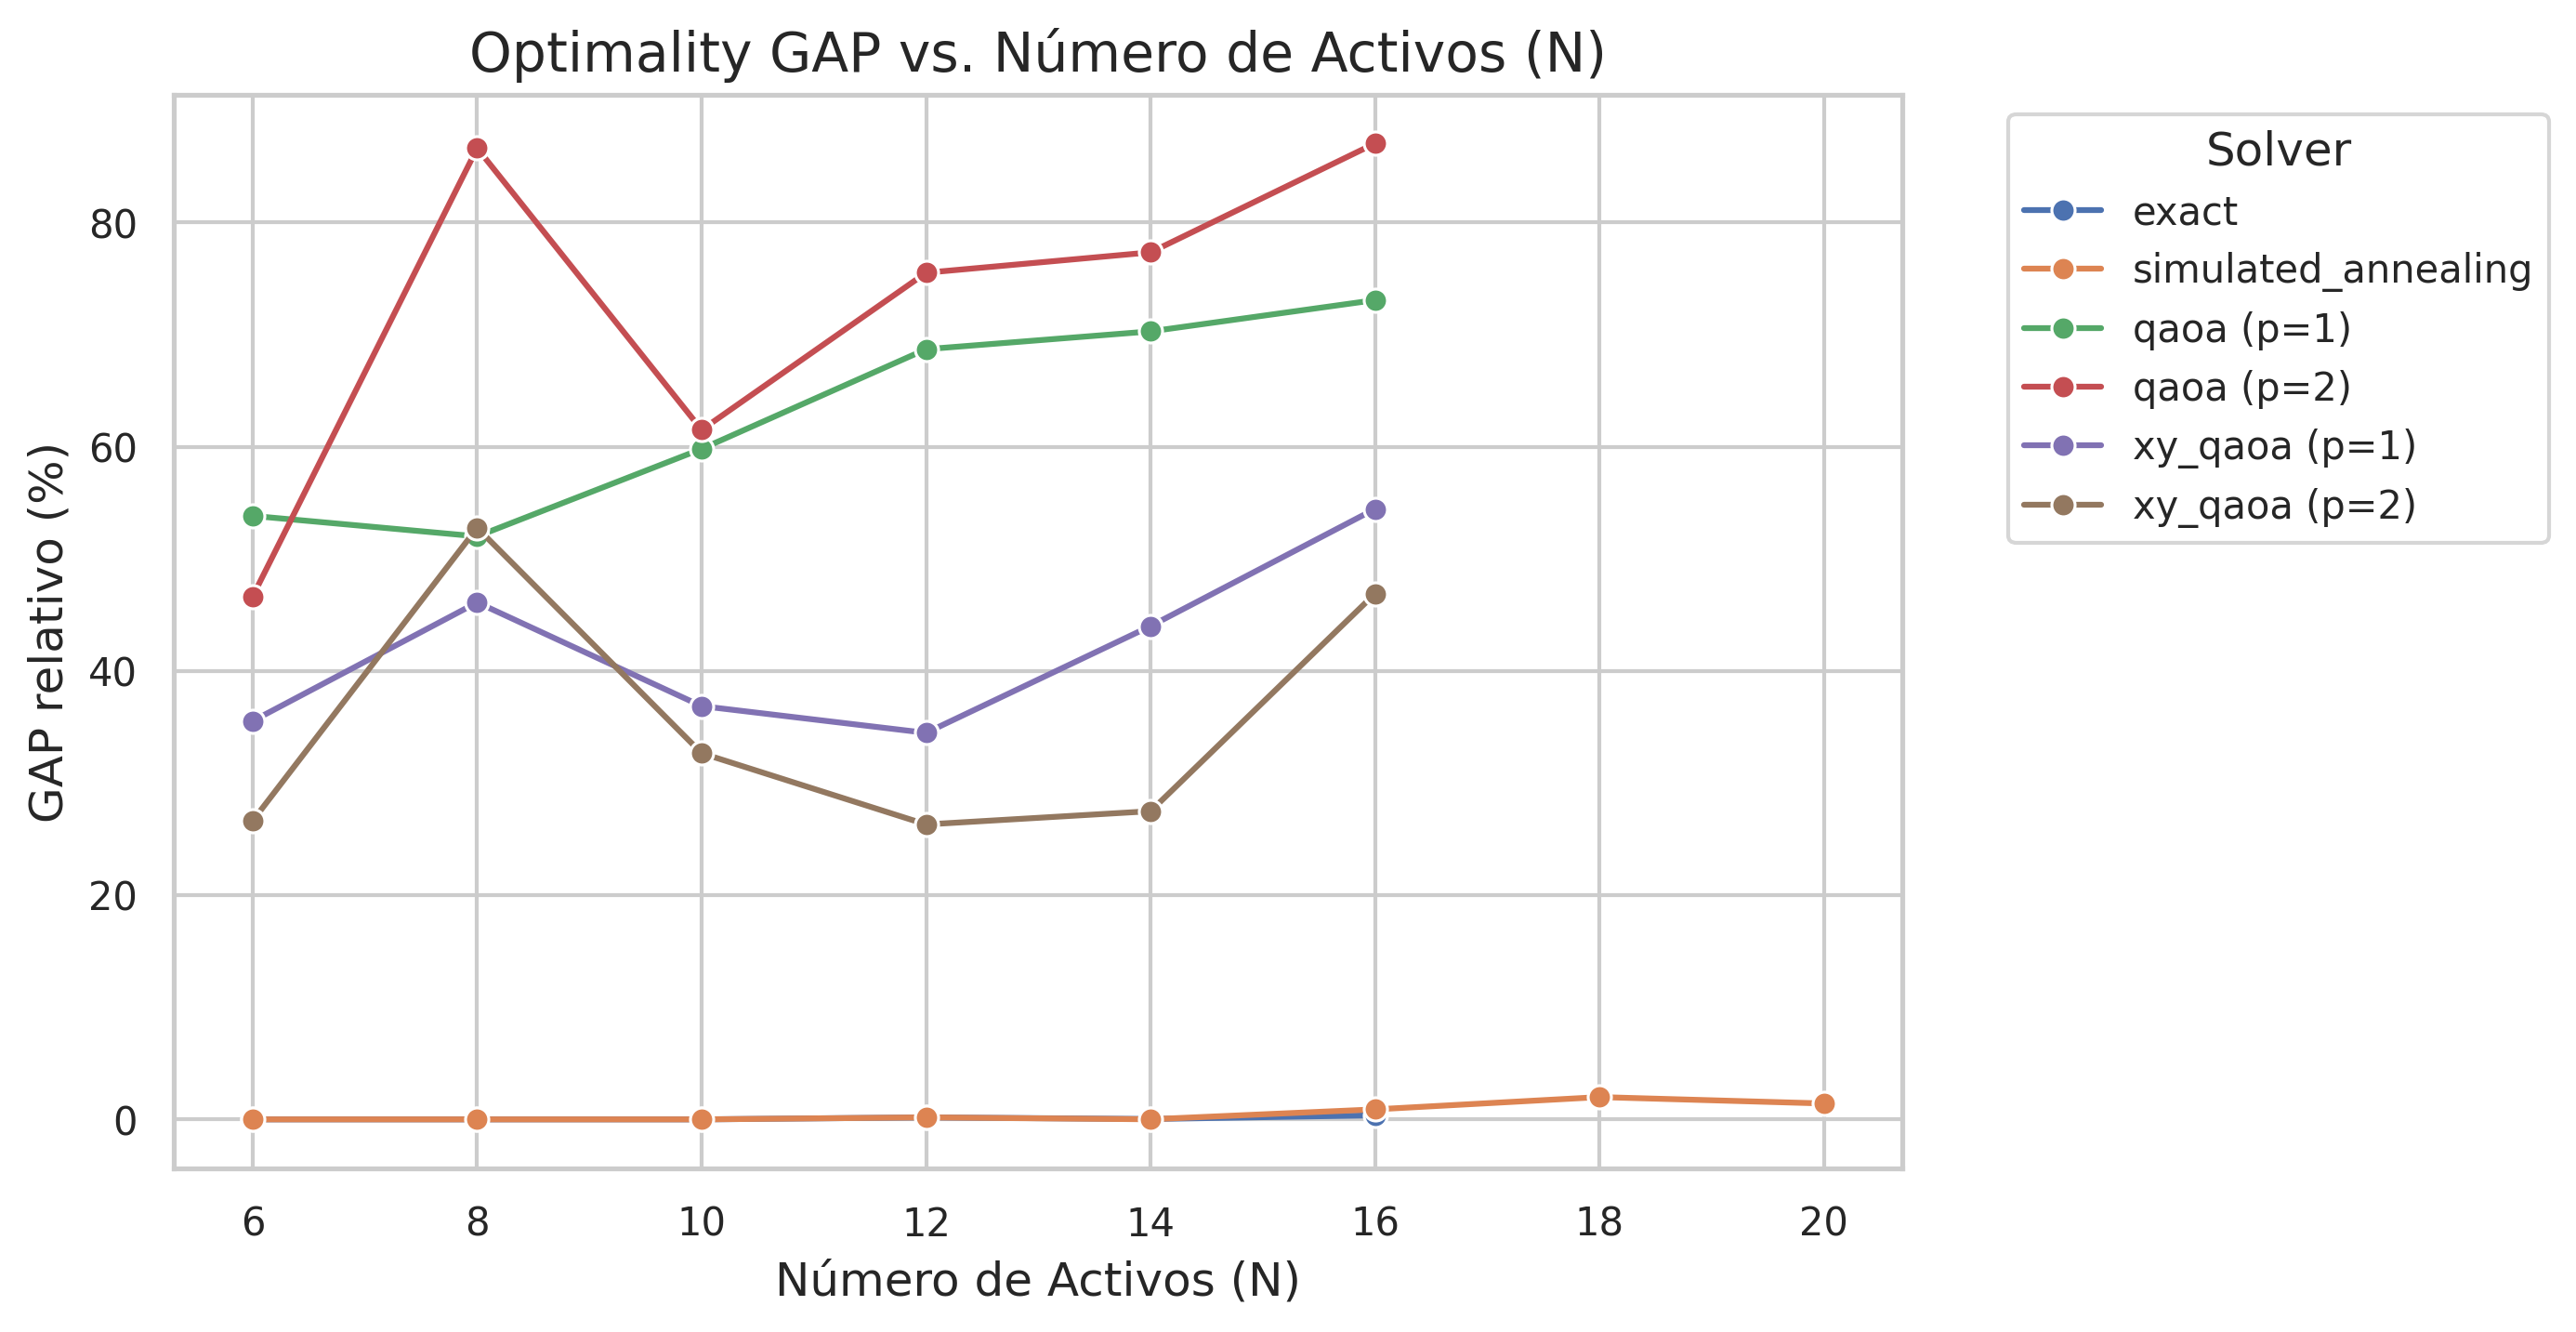
\includegraphics[width=0.85\textwidth]{output/figures/gap_vs_N.png}
    \caption{Evolución del \textit{Optimization GAP} medio en función de $N$. Se destaca el control del error por parte del XY-QAOA Regularizado y el repunte final asociado a los límites de expresividad del circuito a profundidad fija.}
    \label{fig:gap_vs_N}
\end{figure}

\subsection{Impacto de la Profundidad del Circuito ($p$)}
Para validar la hipótesis del límite de expresividad, se procedió a fijar una instancia compleja (ej. $N=14$) y someterla a simulaciones incrementando progresivamente el número de capas o profundidad del circuito ($p$). Como documenta la Figura \ref{fig:gap_vs_p}, la adición de operadores de evolución paramétricos otorga mayor flexibilidad matemática al modelo. Mientras que el QAOA estándar apenas logra escapar de sus mínimos locales (mesetas estériles) al aumentar $p$, el XY-QAOA Regularizado describe una curva de descenso asintótica pronunciada, comprimiendo el GAP empírico a medida que se inyectan nuevas capas, demostrando que la arquitectura diseñada es algorítmicamente capaz de converger al estado fundamental exacto si el hardware permite escalar $p$.

\begin{figure}[htbp]
    \centering
    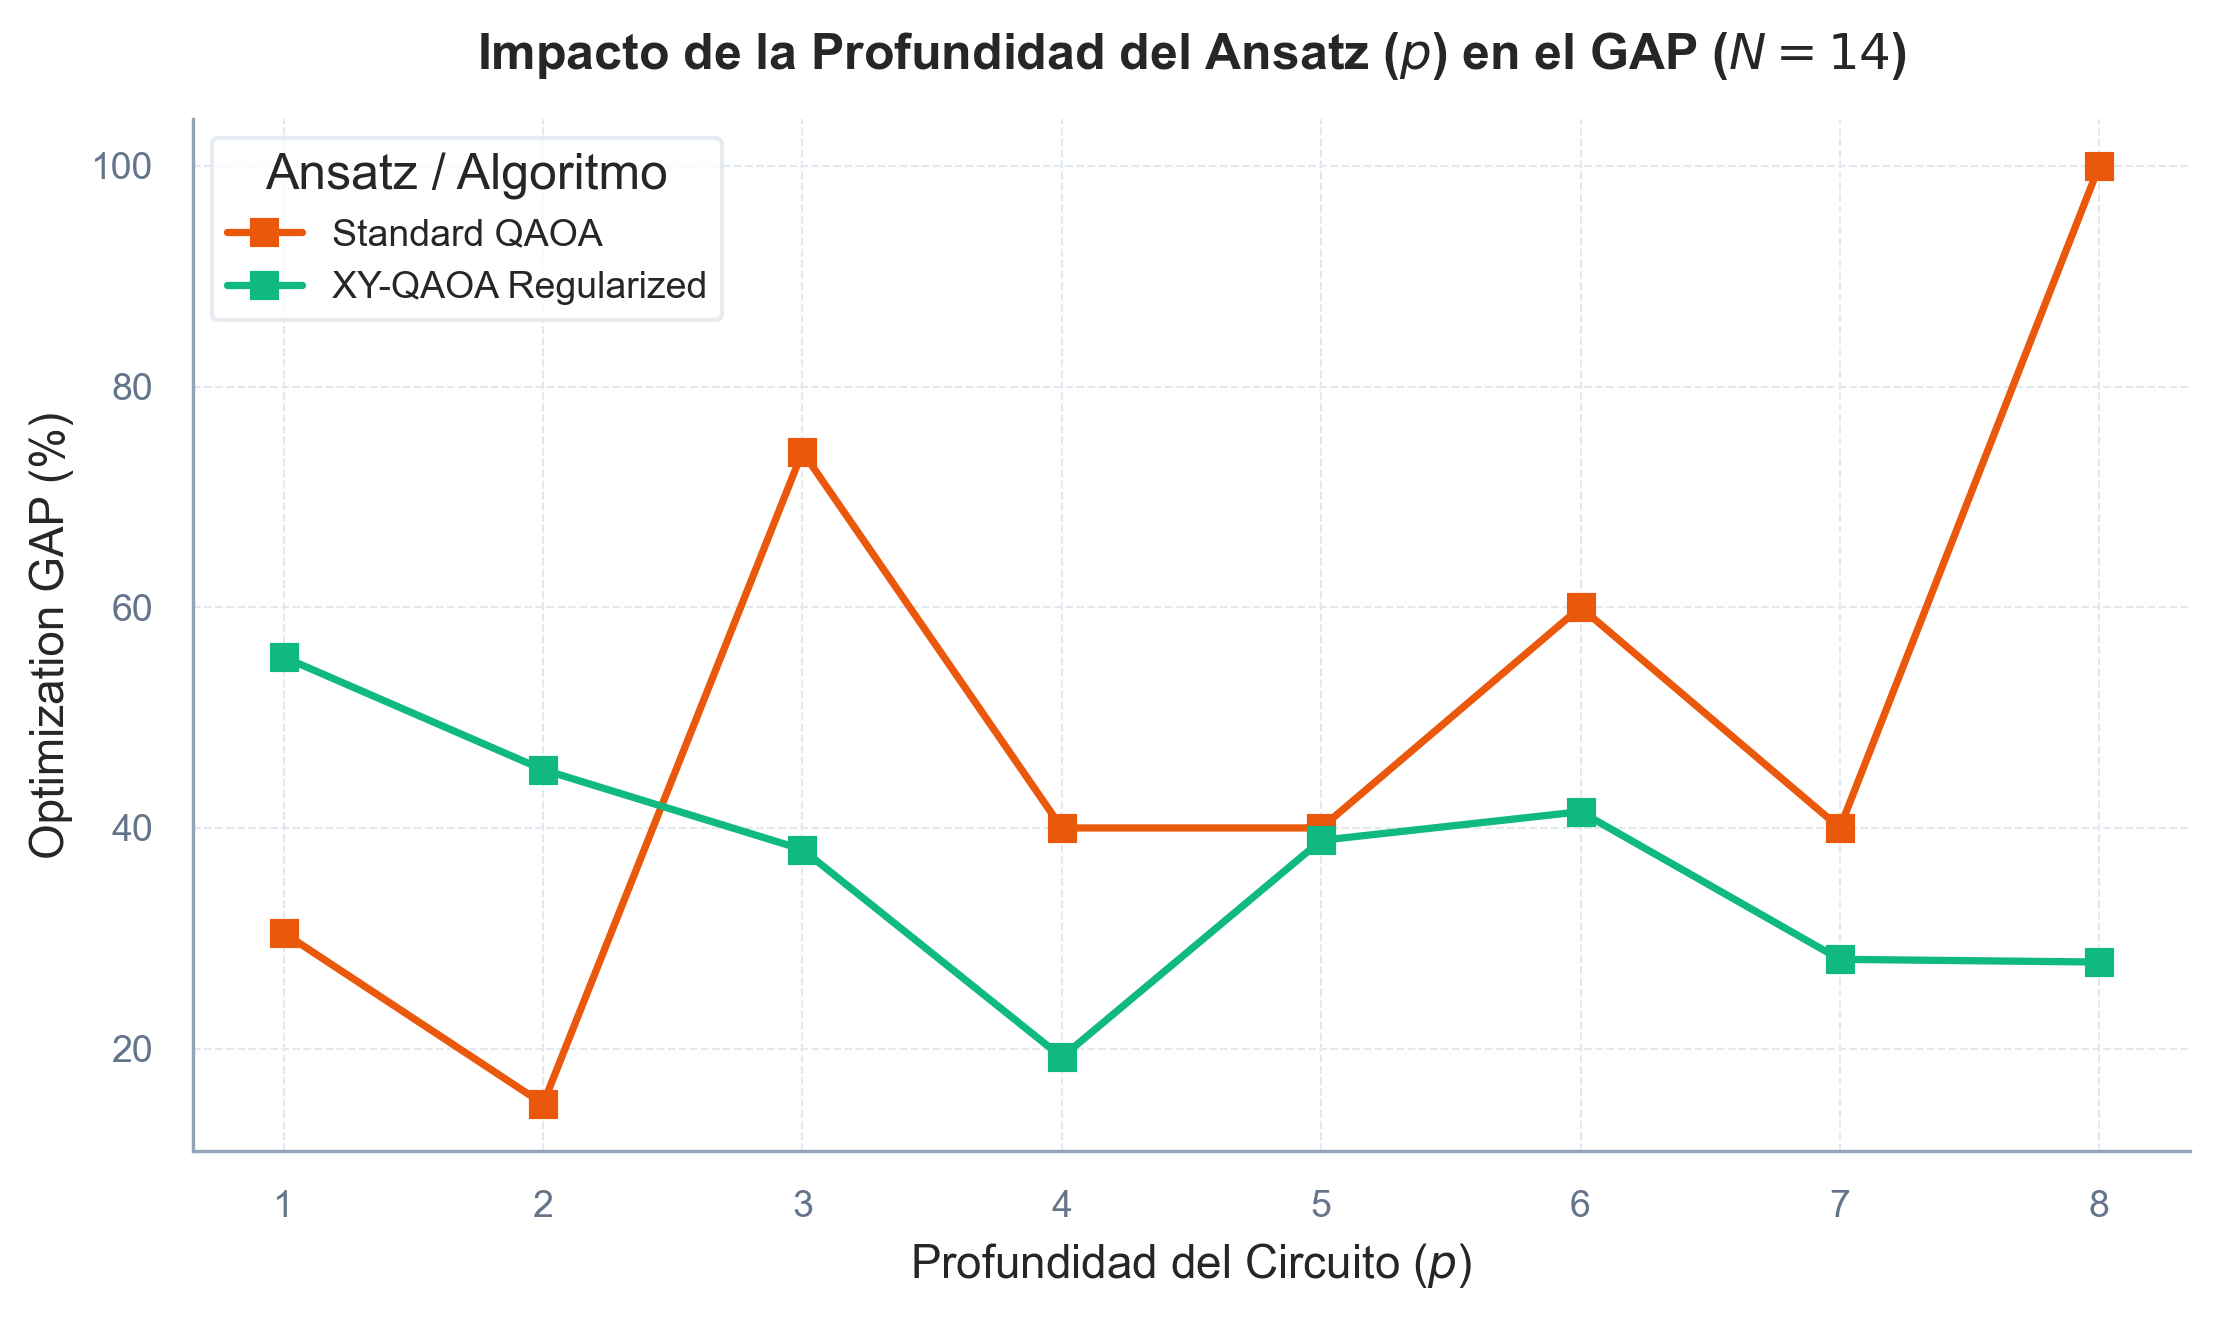
\includegraphics[width=0.85\textwidth]{output/figures/gap_vs_p.png}
    \caption{Impacto del aumento de la profundidad del circuito ($p$) sobre el \textit{Optimization GAP} para una instancia acotada. La arquitectura XY-QAOA exhibe una alta sensibilidad positiva a la inyección de parámetros.}
    \label{fig:gap_vs_p}
\end{figure}

\section{Evaluación Financiera y Robustez del Modelo}
\label{sec:evaluacion_financiera_robustez}

Más allá de la optimización matemática pura, la viabilidad de la tecnología en el sector \textit{Fintech} requiere que las carteras generadas ofrezcan resiliencia en el mundo real. Para ello, se evaluó el Ratio de Sharpe Anualizado en un entorno de validación fuera de muestra (\textit{Out-of-Sample}), exponiendo las carteras optimizadas a datos históricos no vistos durante el proceso de entrenamiento.

La Figura \ref{fig:sharpe_vs_N} revela un comportamiento revelador propio de la modelización financiera. Gurobi, al resolver el problema de manera matemática exacta en los datos de entrenamiento (\textit{In-Sample}), sufre un fuerte castigo por sobreajuste (\textit{overfitting}) cuando las condiciones de mercado cambian en el periodo de test, desplomando su Ratio de Sharpe. En contrapartida, el algoritmo XY-QAOA Regularizado demuestra una notable capacidad de generalización. Al explorar de forma simultánea múltiples configuraciones subóptimas pero altamente diversificadas y estar sometido al suavizado de la regularización Ridge $L_2$, la solución cuántica absorbe mejor el ruido sistémico del mercado, manteniendo un Ratio de Sharpe Out-of-Sample fuertemente competitivo y, en varias instancias, superior al del solucionador determinista clásico.

\begin{figure}[htbp]
    \centering
    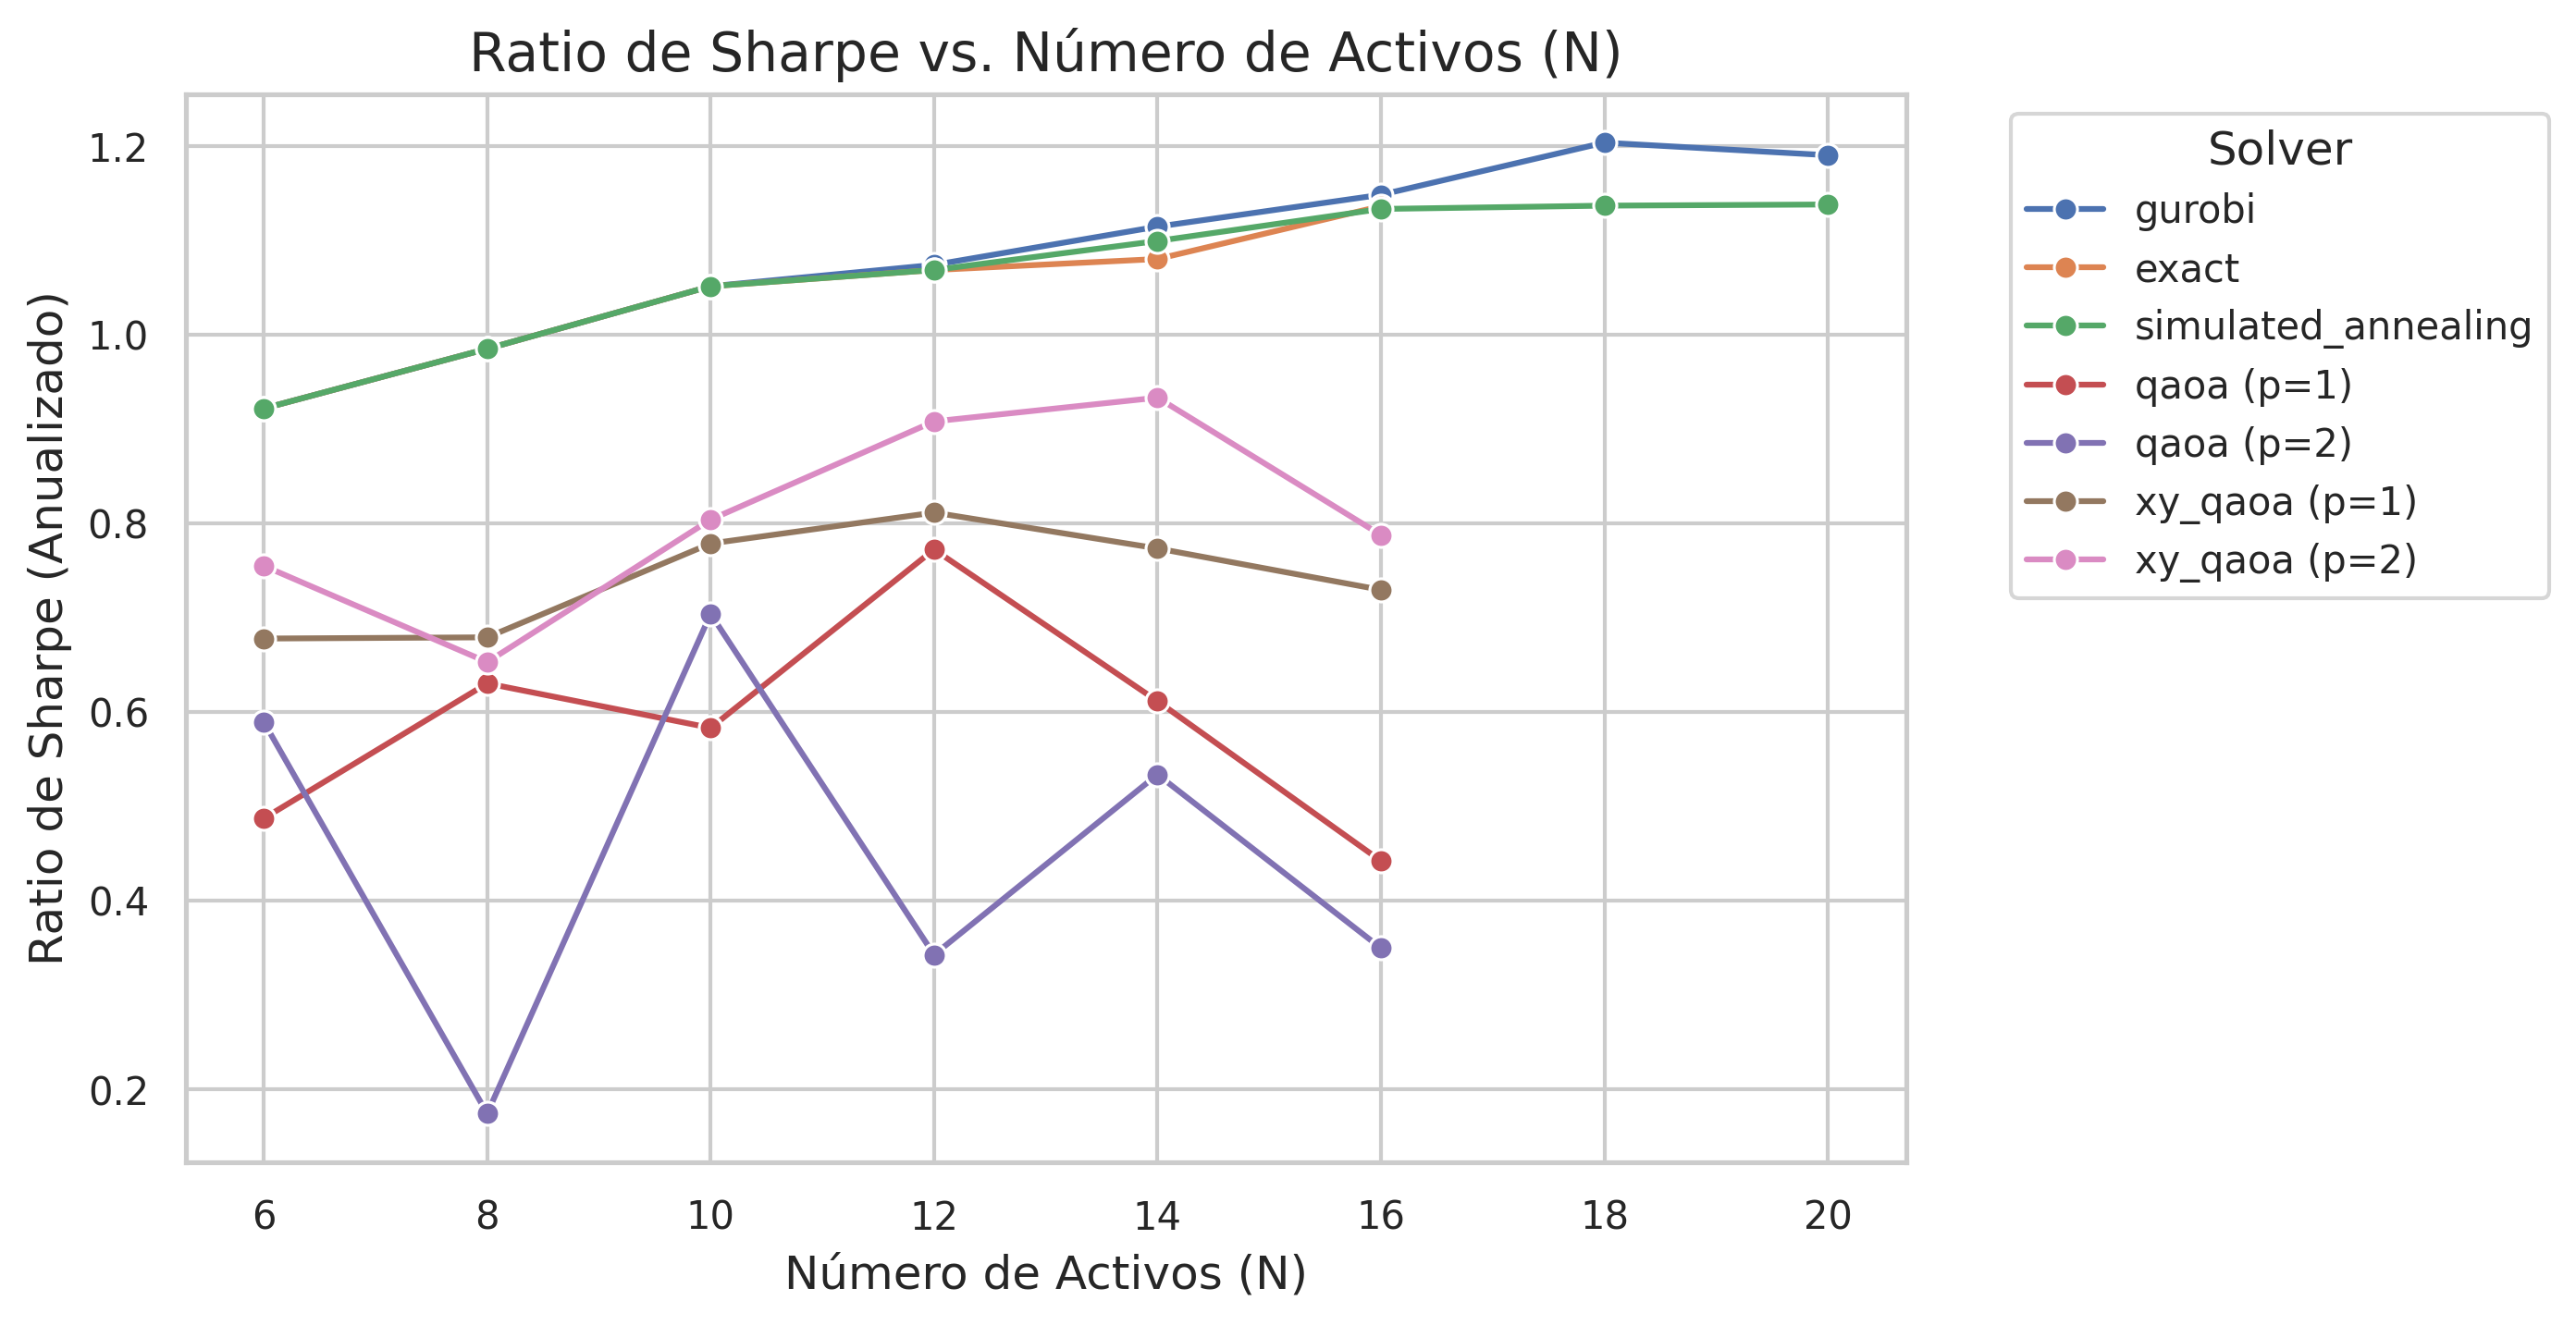
\includegraphics[width=0.85\textwidth]{output/figures/sharpe_vs_N.png}
    \caption{Comportamiento financiero real de las soluciones: Comparativa del Ratio de Sharpe Anualizado. Se evidencia la caída por sobreajuste del solucionador exacto frente a la robustez fuera de muestra del modelo cuántico regularizado.}
    \label{fig:sharpe_vs_N}
\end{figure}

\section{Escalabilidad y Complejidad Computacional}
\label{sec:escalabilidad_complejidad}

El análisis de los tiempos de ejecución pone de relieve el cuello de botella actual de la computación cuántica híbrida durante la era NISQ: la necesidad de emular el entrelazamiento cuántico en hardware clásico.

La Figura \ref{fig:tiempo_vs_N} proyecta el tiempo neto de ejecución computacional. Gurobi y el Recocido Simulado resuelven el problema en fracciones de segundo para escalas bajas, aunque Gurobi comienza a acusar su naturaleza de complejidad exponencial al acercarse a $N=20$. Por el contrario, la simulación del vector de estado del algoritmo cuántico (acelerado mediante JAX) requiere cientos de segundos debido al \textit{overhead} de las operaciones matriciales de tensores. No obstante, el diseño de diferenciación automática permite amortiguar este crecimiento.

\begin{figure}[htbp]
    \centering
    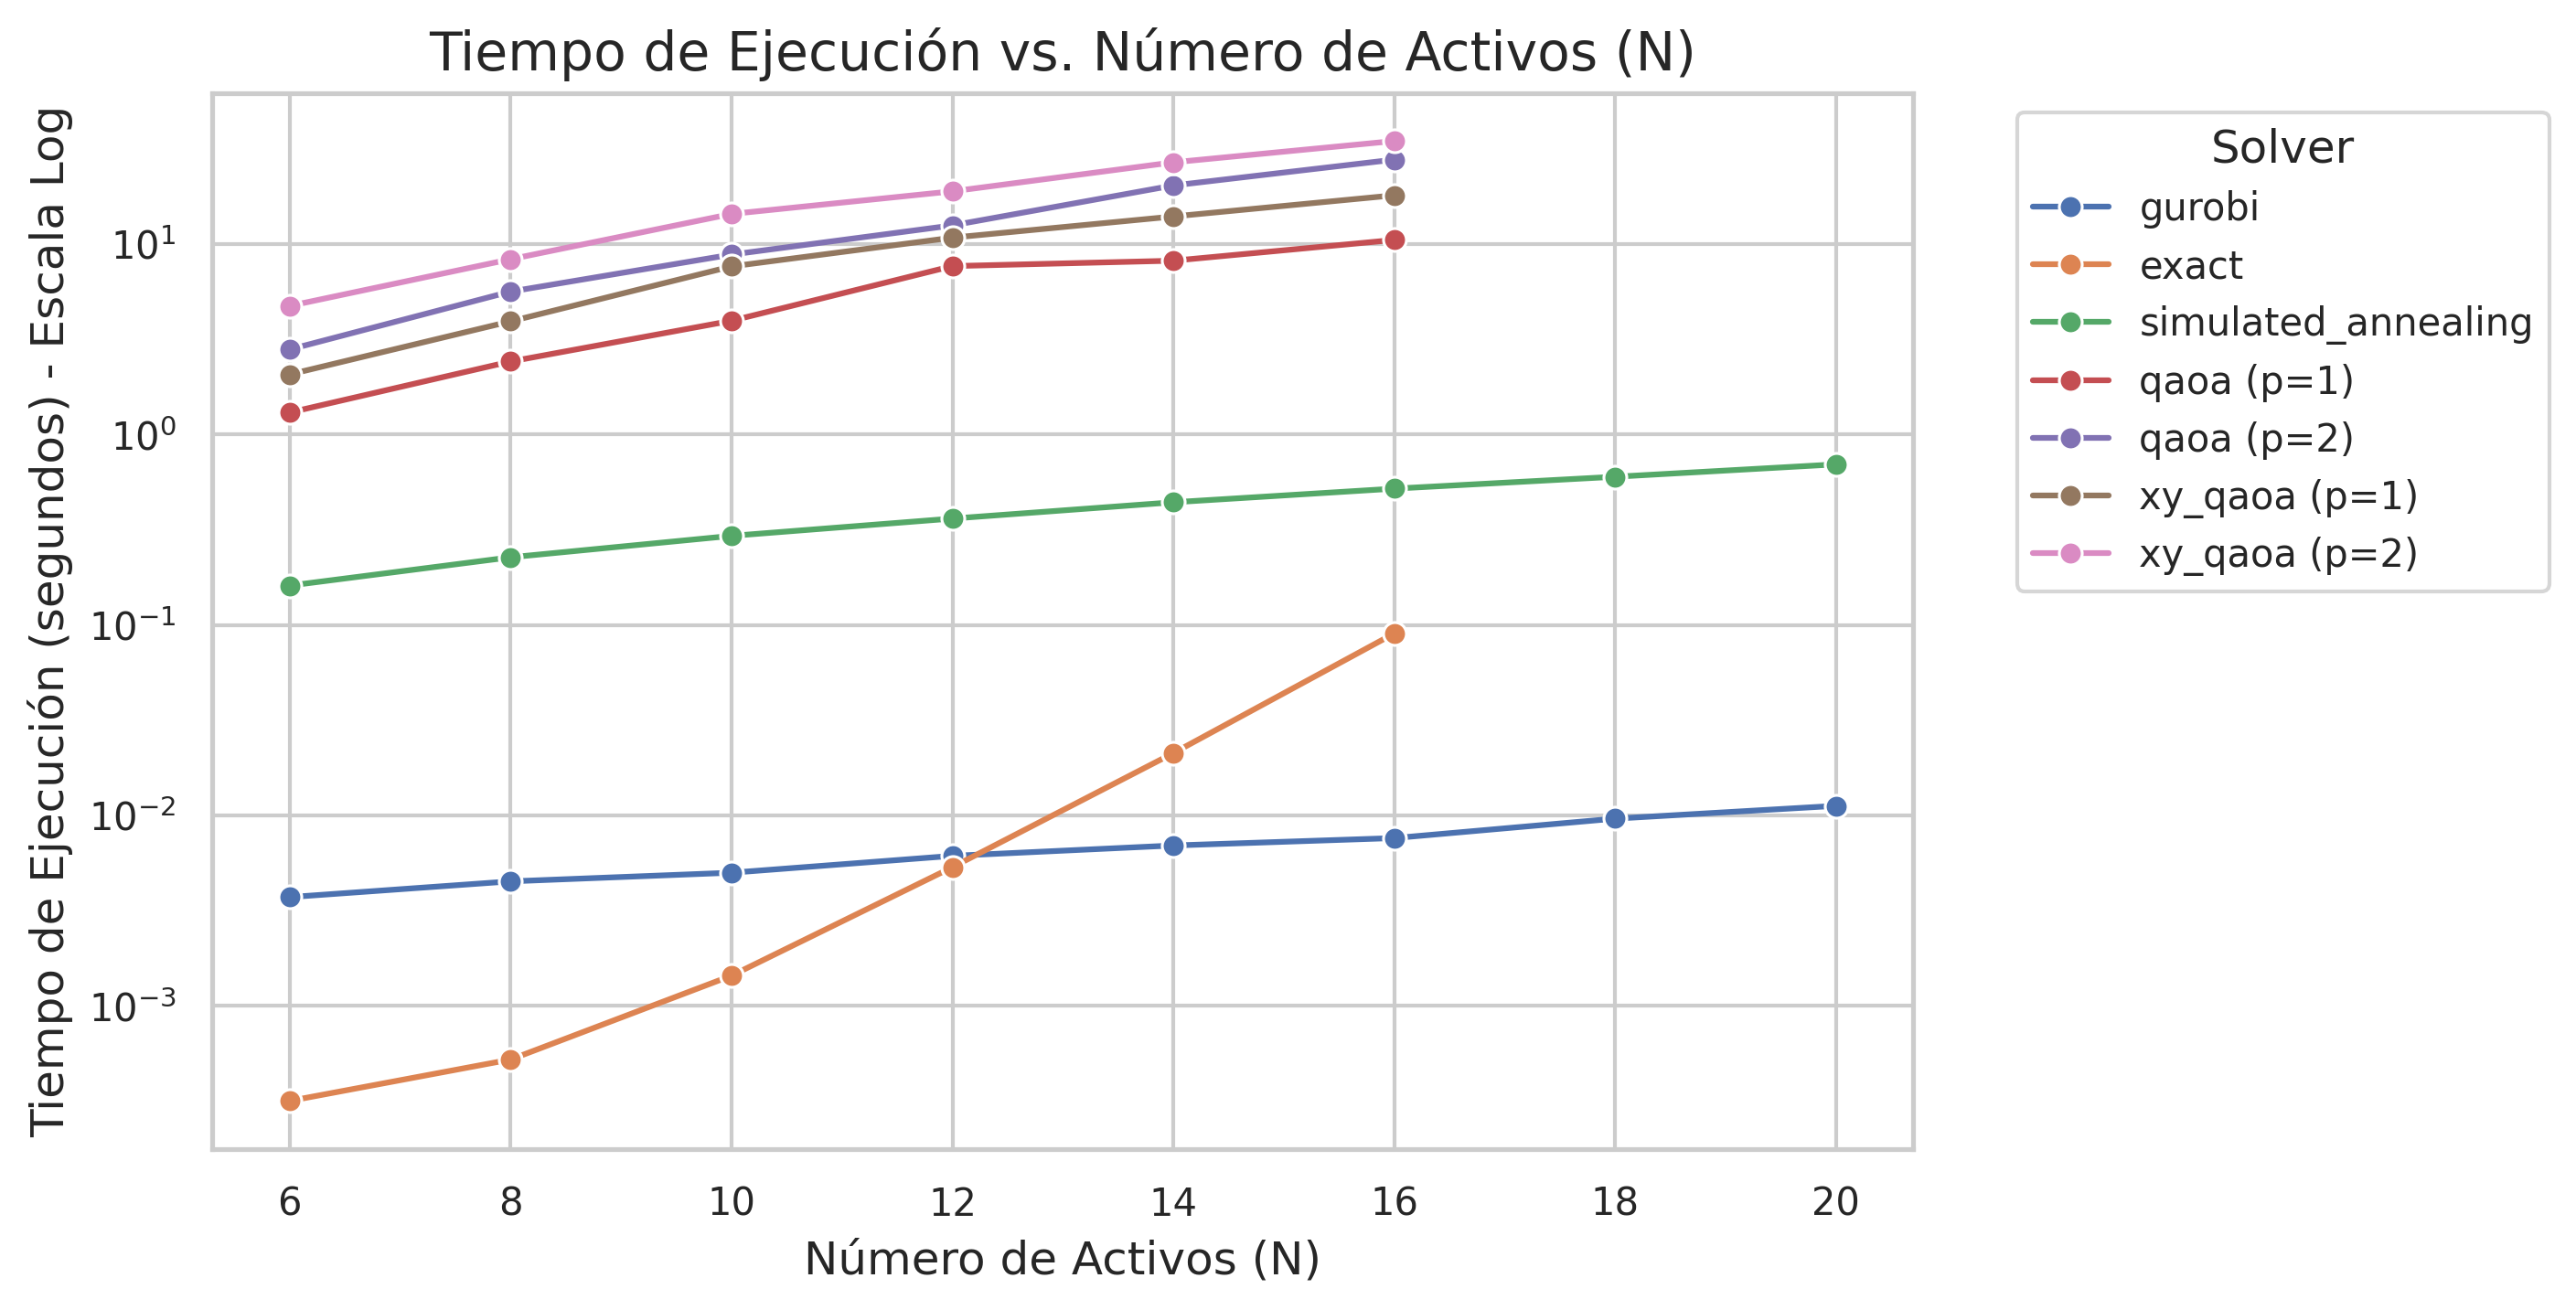
\includegraphics[width=0.85\textwidth]{output/figures/tiempo_vs_N.png}
    \caption{Escalamiento temporal de ejecución (escala logarítmica) en función del universo de activos. La simulación de vectores de estado impone un elevado coste base que contrasta con la rapidez heurística clásica.}
    \label{fig:tiempo_vs_N}
\end{figure}

Por otro lado, la Figura \ref{fig:tiempo_vs_p} aisla el comportamiento interno del simulador variacional frente a la adición de capas cuánticas. Los resultados constatan que, para un tamaño de registro fijo ($N$), el coste temporal del bucle híbrido clásico-cuántico en CPU/GPU escala de forma estrictamente lineal respecto a la profundidad $p$. Este hallazgo certifica la eficiencia de la paralelización lograda en el repositorio desarrollado.

\begin{figure}[htbp]
    \centering
    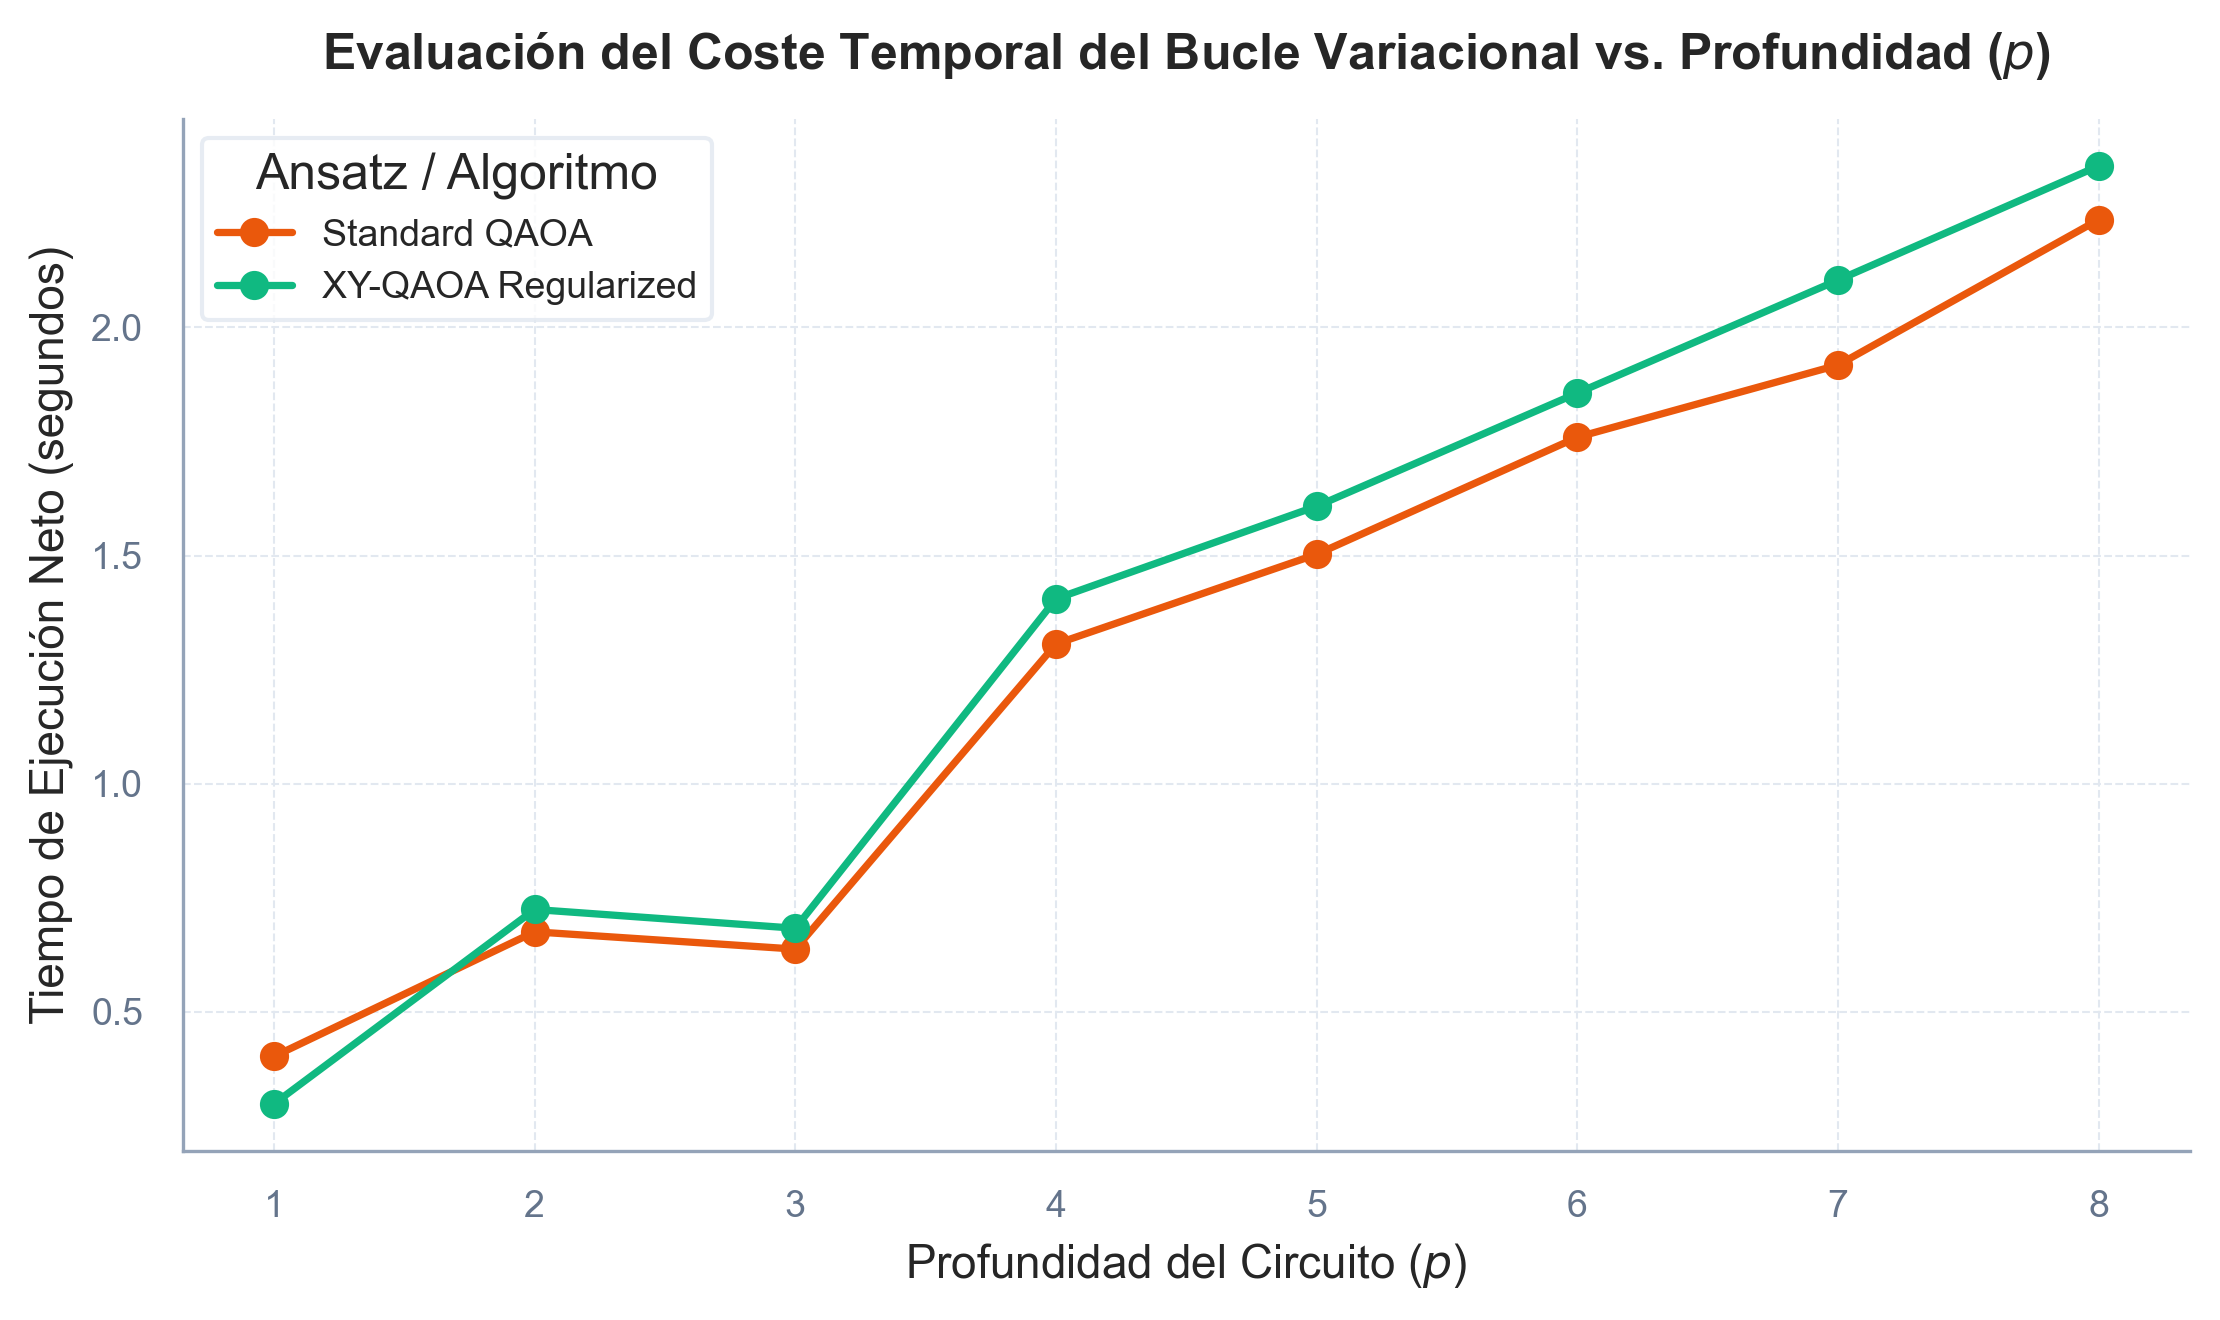
\includegraphics[width=0.85\textwidth]{output/figures/tiempo_vs_p.png}
    \caption{Impacto de la profundidad del circuito ($p$) en el tiempo de procesamiento para distintos volúmenes de activos. Se evidencia un escalamiento lineal de la simulación cuántica respecto a las capas añadidas.}
    \label{fig:tiempo_vs_p}
\end{figure}

\section{Síntesis y Trabajo Futuro}
\label{sec:sintesis_trabajo_futuro}

\subsection{Perfil Multicriterio de los Solucionadores}
Para consolidar de forma visual la toma de decisiones tecnológicas, se ha construido un diagrama de radar (Figura \ref{fig:radar_chart_performance}) que normaliza el rendimiento de los cuatro enfoques principales bajo las métricas de viabilidad, precisión (inversa del GAP), robustez (Sharpe OOS) y eficiencia temporal. 

El diagrama ilustra el \textit{trade-off} central de la optimización cuántica financiera actual: mientras que el XY-QAOA Regularizado domina de forma absoluta en la viabilidad matemática de las carteras y aporta una robustez fuera de muestra sobresaliente comparable a los solvers maduros, se encuentra fuertemente penalizado en el eje de la eficiencia temporal debido a las barreras impuestas por la simulación clásica del hardware cuántico.

\begin{figure}[htbp]
    \centering
    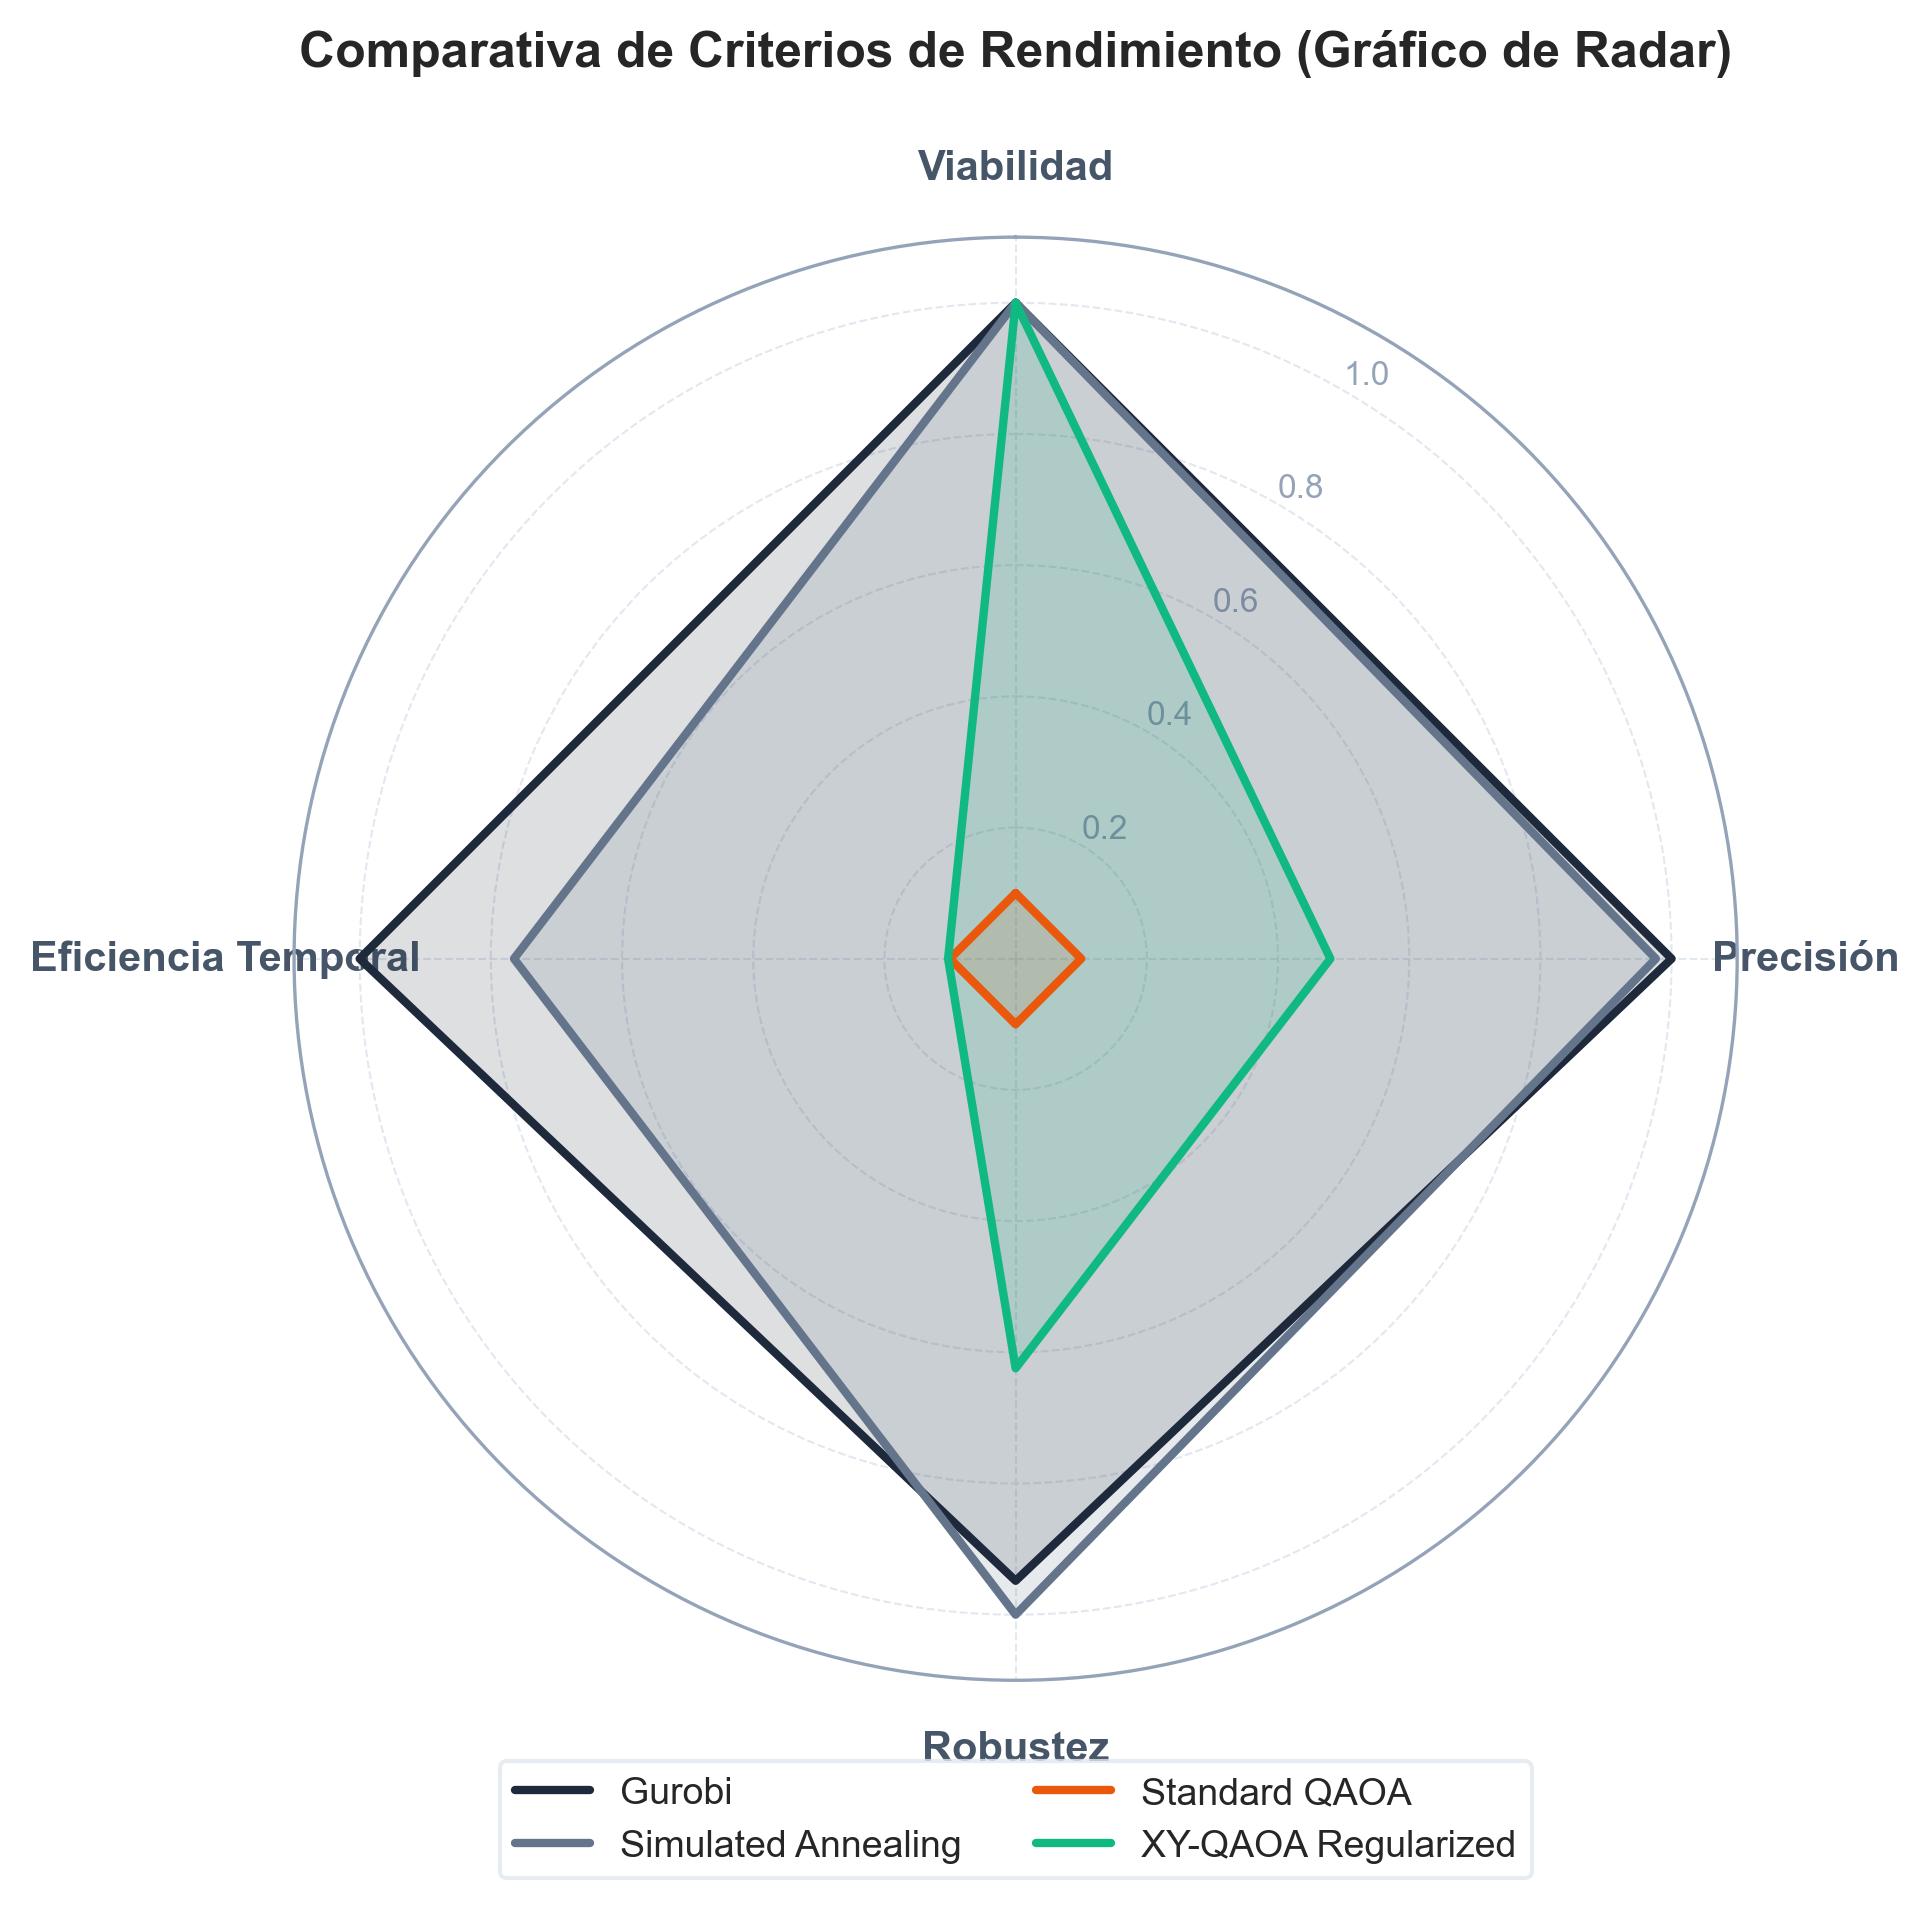
\includegraphics[width=0.85\textwidth]{output/figures/radar_chart_performance.png}
    \caption{Gráfico de radar multicriterio comparando el perfil de rendimiento integral de los solucionadores exactos, heurísticos y cuánticos evaluados.}
    \label{fig:radar_chart_performance}
\end{figure}

\subsection{Conclusiones y Vías de Investigación Futura}
Los resultados obtenidos certifican la consecución de los objetivos de la investigación. Se ha demostrado empíricamente que la sustitución de las inestables penalizaciones QUBO por confinamientos geométricos (XY-Mixer) resuelve el problema de la viabilidad de la cardinalidad de manera definitiva. A su vez, el marco de regularización introducido dota a la optimización clásica de la estabilidad necesaria para generar soluciones financieras competitivas frente al sobreajuste de los modelos exactos deterministas.

No obstante, en base a la evidencia arrojada por los tiempos de ejecución y las exigencias de expresividad, se concluye con honestidad científica que en la actual era NISQ no existe ventaja cuántica operativa para el problema de carteras con $N \le 20$ activos. El trabajo futuro deberá orientarse inexcusablemente hacia dos vectores:
\begin{enumerate}
    \item \textbf{Mitigación de Errores de Hardware:} Integrar en el \textit{pipeline} técnicas de extrapolación de ruido (ZNE) para permitir que el circuito transpilado en topologías lineales físicas absorba las altas tasas de error de las compuertas de intercambio subyacentes.
    \item \textbf{Despliegue FTQC:} Trasladar la arquitectura base de este repositorio, ya depurada matemáticamente, hacia procesadores de la era de computación cuántica tolerante a fallos, donde escalar $p$ para solventar la explosión combinatoria no implique la destrucción de la coherencia del estado.
\end{enumerate}